\documentclass[parskip=full]{scrartcl}
\usepackage[utf8]{inputenc} % use utf8 file encoding for TeX sources
\usepackage[T1]{fontenc}    % avoid garbled Unicode text in pdf
\usepackage[english]{babel}  % english hyphenation, quotes, etc
\usepackage{hyperref}       % detailed hyperlink/pdf configuration
\hypersetup{                % ‘texdoc hyperref‘ for options
pdftitle={HePICS Design Document},%
bookmarks=true,%
}
\usepackage{graphicx}       % provides commands for including figures
\usepackage{csquotes}       % provides \enquote{} macro for "quotes"
\usepackage{enumitem}


\title{HePICS Design Document}

\begin{document}

\maketitle
\thispagestyle{empty}
\pagebreak





\tableofcontents
\pagebreak





\section {Functionality Description}

In model part, the classes realize the management of all the data and logic. They load the path of images and access their features. The results of classification are stored in the type of string to be shown in various forms. The logic of classification is determined by the neural network being used. Its topology defines how different layers interact with each other. With the assistance of all the layers, the forward propagation functionality can be implemented, which is the core of algorithms for image classification with pre-trained model.

The view realizes the user interfaces. The welcome window and the main window, which contains three different sections, guide the user to upload their input files, select available platforms and operating mode, let them control the process and show the prediction results. 

The controller accepts user inputs handled by the components of the views and converts them to the commands. The classifier controls the progress of processing and assigns the scheduler to dispatch work to workers in heterogeneous platforms. In addition, the poller checks the requests from external systems regularly. After receiving the correct request with the image path, the classifier starts the process of classification.

\section {Class Diagram Description}

In this diagram seveal design patterns were used.
In order to decouple  major components and allow parallel development we use the Model-View-Controller as a global architecture.
The class diagram consists of several common patterns to reduce complexity and dependencies between classes.
We use the template Method as pattern for sections to define the skeleton of the algorithm in an operation.
However the results and states are updated using an observer which define a one-to-many dependency between objects.
Different Modes as well as Worker are represented by simple is-relationships.
Another interesting pattern to be used by layers is the strategy-pattern. In this context we define a family of algorithm, encapsulate
each one and make them interchangeable.This approach also lets the algoritm vary independently from the layer that use it.

\pagebreak

\section {Class Description}

HepicsGui: represents the main entry point to execute the software. It contains the main Method.

WelcomeWindow: This class is used to display informations about the developed software.

MainWindow: is the main class that runs the classification system. It is also responsable for setting up the GUI.

Section: creates a label for each part of the GUI. Suclasses define sections (e.g. buttons, check boxes) and handle their actions.

ImageSection: allows the user to add and delete input images.

Plattform\_Mode\_Section: allows the user to choose operation mode and a platform to run the classification or aggregation on it.

ControlSection: allows the user to start, pause, resume and cancel the classification process.

Observer: defines an updating interface for objects that should be notified of changes in a subject.

ObserverManager: provides an interface for attaching and detaching Observer objects. It notifies concrete observers whenever corresponding data changes.

ResultObserver, StateObserver: implement the Observer updating interface to keep its state consistent with concrete subjects and maintain reference to those subjects.




Image : is an abstract class which represents the modelisation of an image in the programming language. Its attributes are length, width, channel, and id, which means each uploaded or created image is unique. This class is only a representation of an image object, it can be replaced by an existing library.

InputImage : represents an input image. Has an extra attribute isClassified, which tells if the image has already been classified. In this case, it is not necessary to redo the classification. It is also possible to create a thumbnail out of this image.

ResultImage : represents the image that is displayed which contains the results of the classification. It has an extra attribute called result, which is a string containing the results. These results can also be displayed in other ways if it is wished to extend the functionality of the system (histograms, pie charts)

ImageManager : is responsible of providing the input image to the system and its preprocessing, which means, converting it into a matrix, or an RGB image, depending on what the process needs.

DataSaver : saves the input images loaded during all the time the system has been running in a hashmap. Can also write the results in a text file, and aggregate the results of the given inputs.

ClassificationAssistant : is practically the classifier's secretary. It makes sure that the classifier gets all what it needs to run the classification. It loads weights, sets the input image in the wished form, and loads all the neural networks needed specifications, as well as the classification's class names.

NeuralNetwork : is the modelisation of a neural network. A neurel network has a name, a topology and a set of layers.

Shape : contains constants which define the form and general composition of a layer.

Topology : is the visual representation of the neural network, meaning the layers and the relations or interactions between them.

TopologyDisplayer : is a tool which is responsible of drawing the representation of the topology and generating an image.

Layer : is what a neural network is made of. It is a set of nodes placed on each other which each treat the input image depending on their type and activation function.




InputLayer Class: This class is the first layer of a neural network (the input layer), it is followed by one or more hidden layers.  It has an Attribut shape wich will be used for the first layer.

Abstract ConvolutionalLayer Class: In this class convolutional layer the input keeps its original shape in order to exploit this correlation between the pixels. A filter will be used in this context in order to convolve input and a stride controls how the filter convolves around the input volume

CPUConvolutionalLayer Class: this class inherits from the Abstract ConvolutionalLayer Class. It uses the CpuWorker in order to do computation.

FPGAConvolutionalLayer Class: this class inherits from the Abstract ConvolutionalLayer Class. It uses the FpgaWorker in order to do computation.

MaxPoolLayer Class: These layer take the output feature, maps from the convolutional layers, and its Max function is to reduce the size of the input feature maps to reduce the amount of parameters in the network.
The pooling layer works in a similar way to the convolutional layer since it operates on a subregion on the input feature maps and performs a filter operation.

ResponseNormalizationLayer Class: The Class Response Normalization is kept separate from the others since it may require multiple memory access patterns.

DenseLayer Class:  this layer can use convolutional blocks for calculations, both of them have access to these blocks.

TrainableLayer Class: this class trains the neural network using a weight matrix

ActivationFunction Class:  Activation function is introduced, its purpose is to allow small changes in the weights or bias to only cause a small change on the output, this property is helpful when training a network.

Sigmoid Class:  $g(z) = 1 / (1 + e^{-z})$ It’s used on the output layer so that we can easily interpret the output as probabilities since it has restricted output between 0 and 1.
sigmoid is an activation function.  Same as the linear classifier this network also has ten outputs since it is the same classification problem, however the hidden layer has 25 neurons.

Tanh Class: $g(z) = (e^z -e^{-z}) / (e^z + e^{-z})$ It’s superior to sigmoid function in which the mean of its output is very close to zero, which in other words center the output of the activation units around zero and make the range of values very small which means faster.

Sofmax Class: It generates a value between 0–1 for each node (the sum of all these softmax values is equal to 1). We can interpret the softmax values for a given image as relative measurements of how likely it is that the image falls into each target class.

ReLU Class:  g(z) = max{0, z}. The models that are close to linear are easy to optimize. Since ReLU shares a lot of the properties of linear functions, it tends to work well on most of the problems.

LayerType : is an enumeration class of the possible layer types.




FileLoader: A dialog used to open files.

LayerType: Defines a constatnt for every type of layer.

Mode: An interface for classification modes. It has methods for different workers.

HighPerformanceMode: A class that implements the methods of interface Mode. Its methods are optimized for high performance.

LowPowerMode: A class that implements the methods of interface Mode. Its methods are optimized for low power.

EnergyEfficiencyMode: A class that implements the methods of interface Mode. Its methods are optimized for energy efficiency.

WorkUnit: An interface for units of work.

ImageLoadWorkUnit: Implements a unit of work for loading images.

LayerWorkUnit: Implements a unit of work for calculating a Layer of the neuronal network.

Scheduler: The Scheduler uses the mode to decide which work unit to use next. The mode is set by the respective methods. The Scheduler also holds the RessourceManager. It is able to control the execution and report about its progress.

RessourceManager: Manages ressources for classification. The only ressource at the moment is a counter for files.

Classifer: Controls the classification. Holds the Workers. It creates and deletes workers based on which platforms are enabled.

Poller: A class for polling a file. The file gets requests for classification. The class extracts the requests.

Worker: The abstraction of a worker. Uses a thread for execution.

GpuWorker: A class implementing the worker for GPU usage.

FileLoadWorker: A class implementing the worker for loading files.

CpuWorker: A class implementing the worker for CPU usage.

FpgaWorker: A class implementing the worker for FPGA usage.



\pagebreak

\section {Diagrams}

\subsection {Overview Sequence Diagram}

\begin{center}
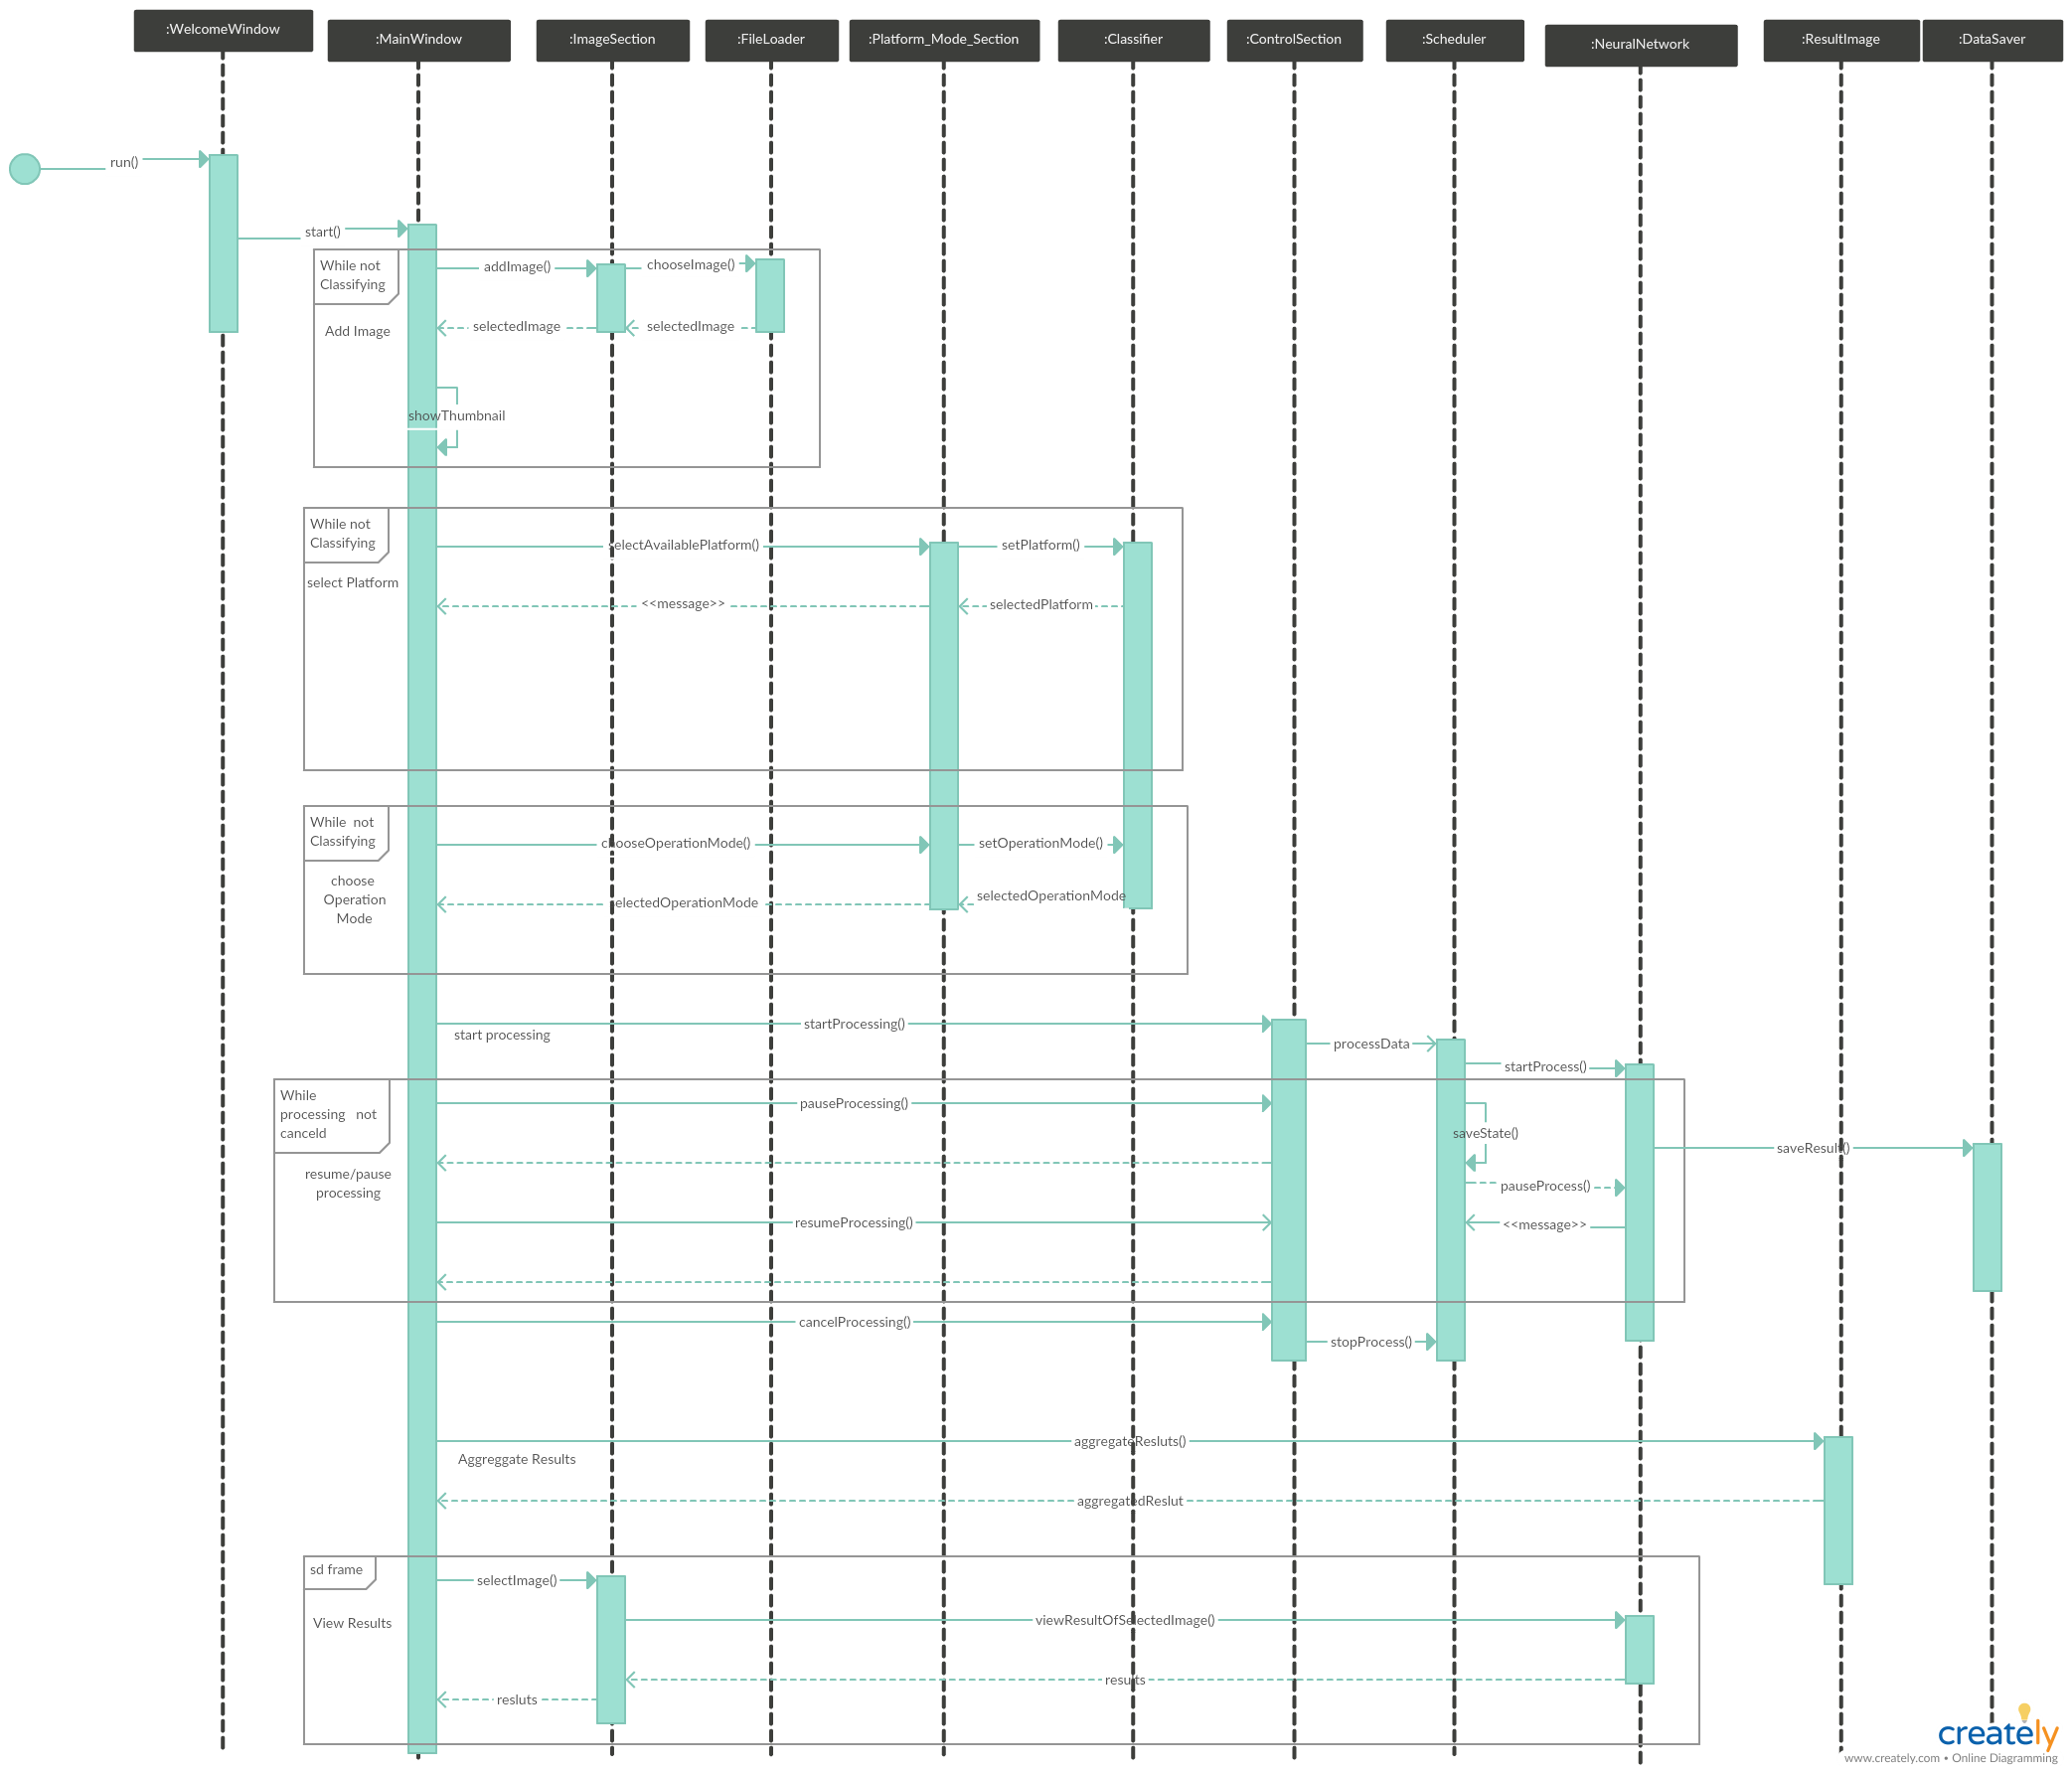
\includegraphics[width=1.0\textwidth]{seq.png}
\end{center}

\pagebreak

\subsection {Select Platforms Sequence Diagram}

\begin{center}
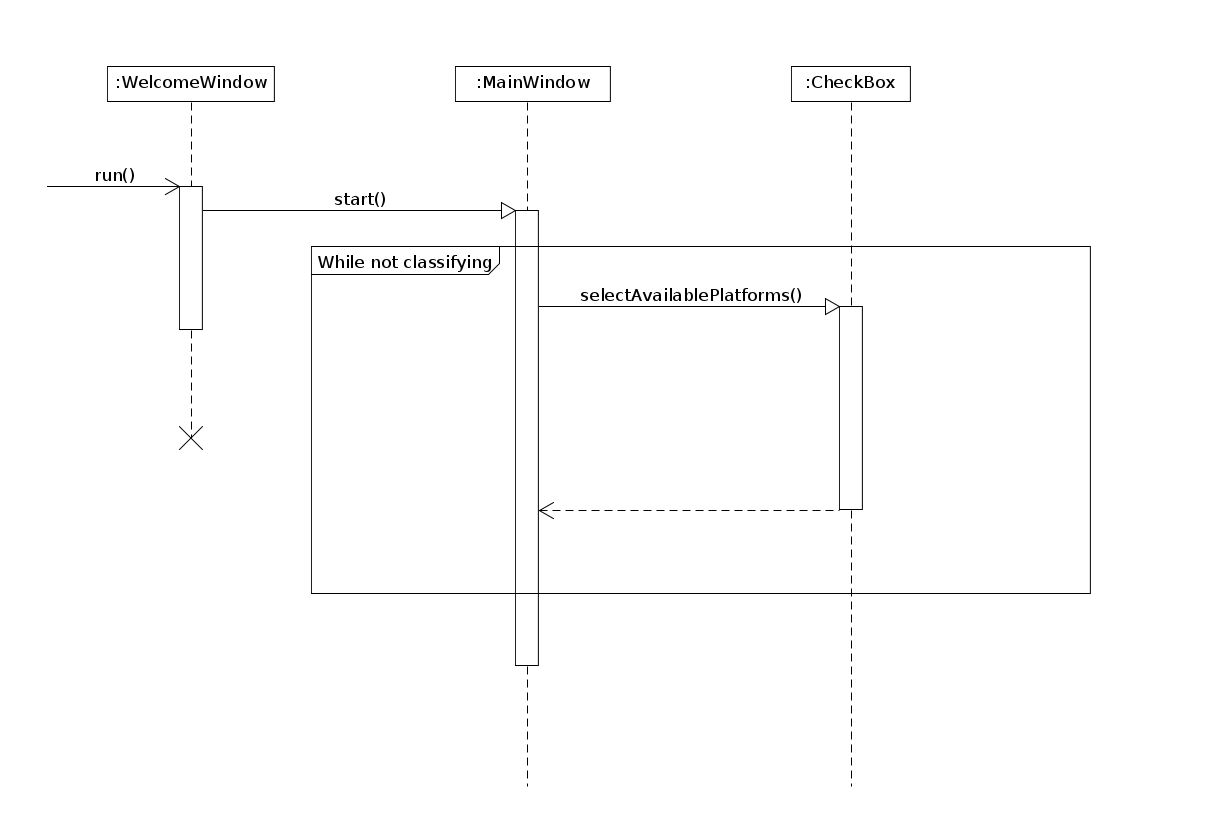
\includegraphics[width=1.0\textwidth]{SelectPlatforms.jpg}
\end{center}

\subsection {Select Image Sequence Diagram}

\begin{center}
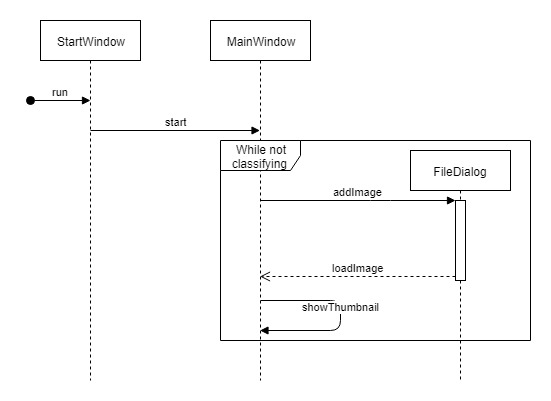
\includegraphics[width=1.0\textwidth]{SelectImageSeqDiag.jpg}
\end{center}

\pagebreak

\subsection {Classification Sequence Diagram}

\begin{center}
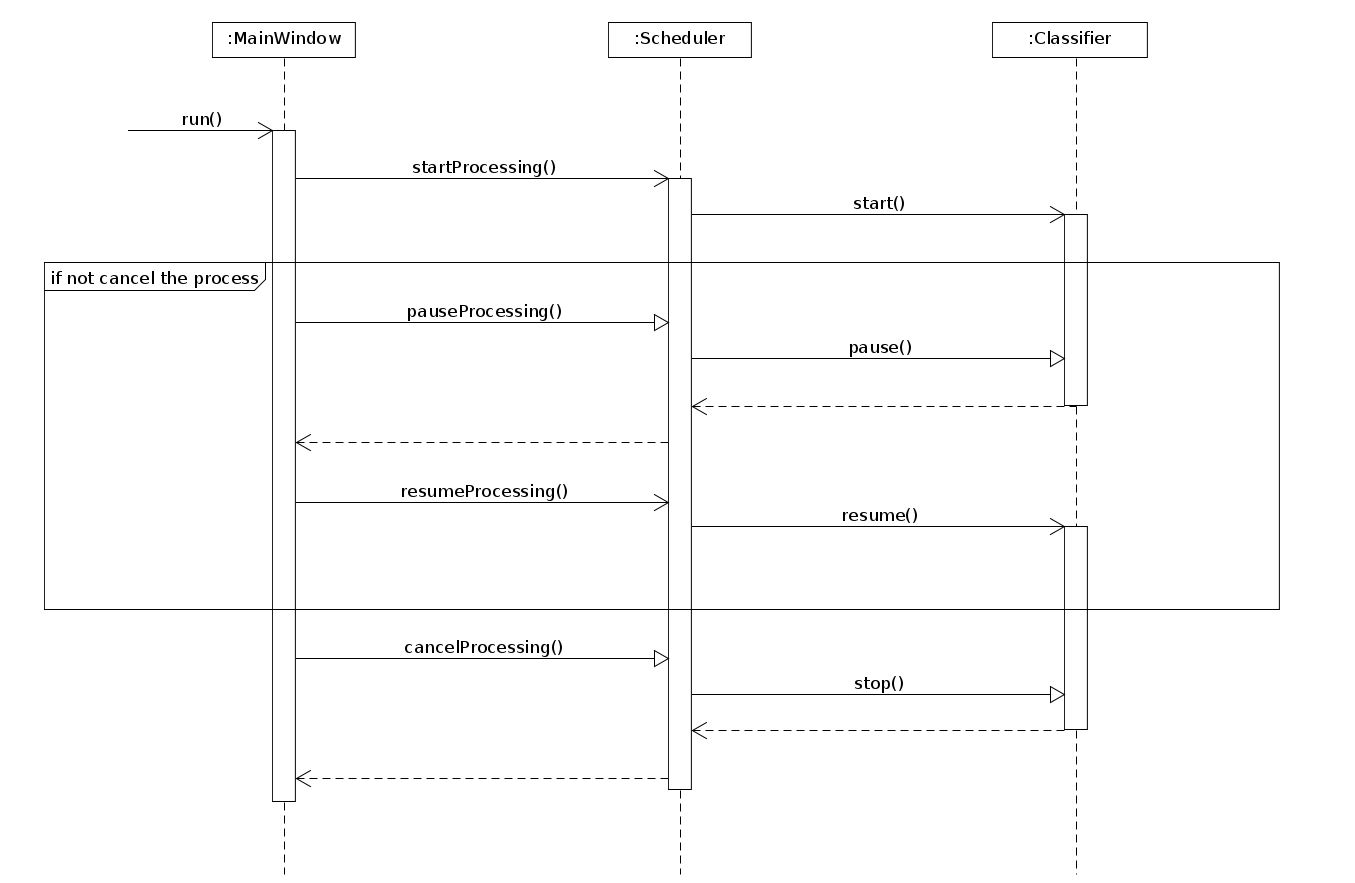
\includegraphics[width=1.0\textwidth]{Classification.jpg}
\end{center}

\pagebreak

\subsection {View Results Sequence Diagram}

\begin{center}
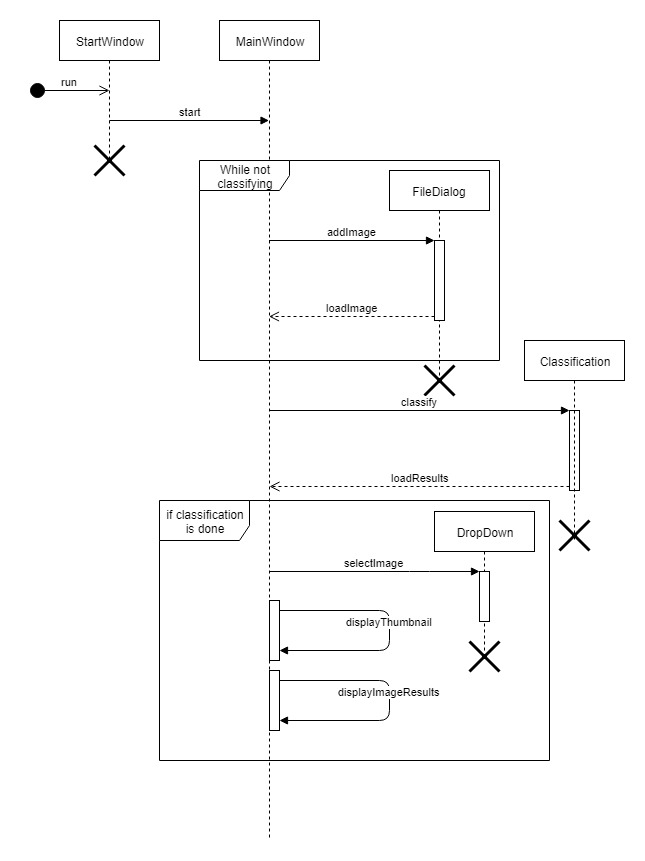
\includegraphics[width=1.0\textwidth]{ViewResults.jpg}
\end{center}

\pagebreak

\subsection {Aggregate Sequence Diagram}

\begin{center}
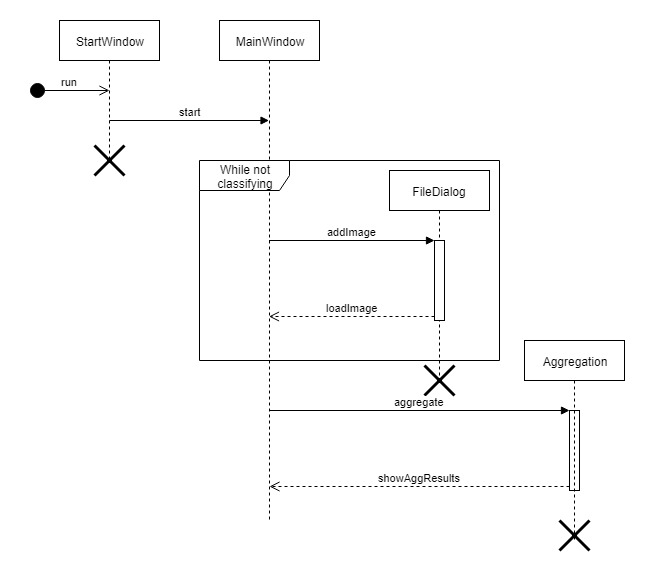
\includegraphics[width=1.0\textwidth]{Aggregate.jpg}
\end{center}

\pagebreak

\subsection {Select Operation Mode Sequence Diagram}

\begin{center}
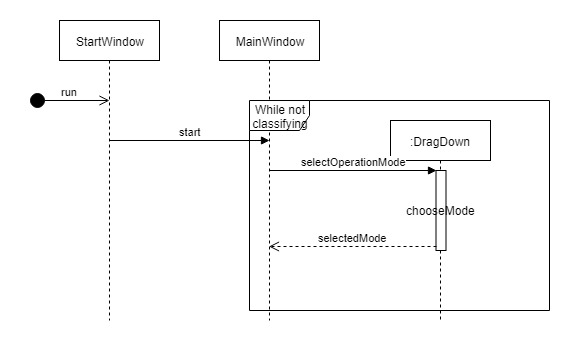
\includegraphics[width=1.0\textwidth]{SelectOperationModeSequenceDiag.jpg}
\end{center}

\pagebreak

\subsection {External Use Sequence Diagram}

\begin{center}
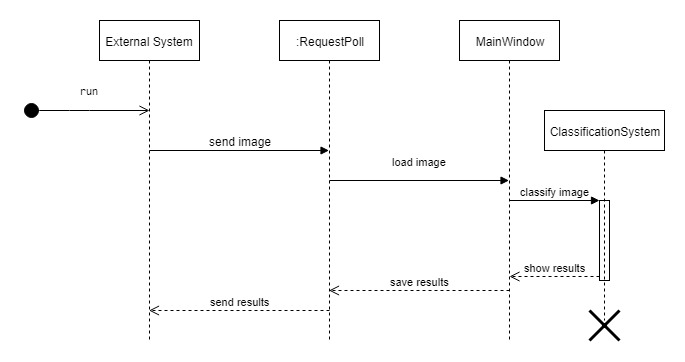
\includegraphics[width=1.0\textwidth]{Untitled Diagram.jpg}
\end{center}

\pagebreak

\subsection {State Diagram}

\begin{center}
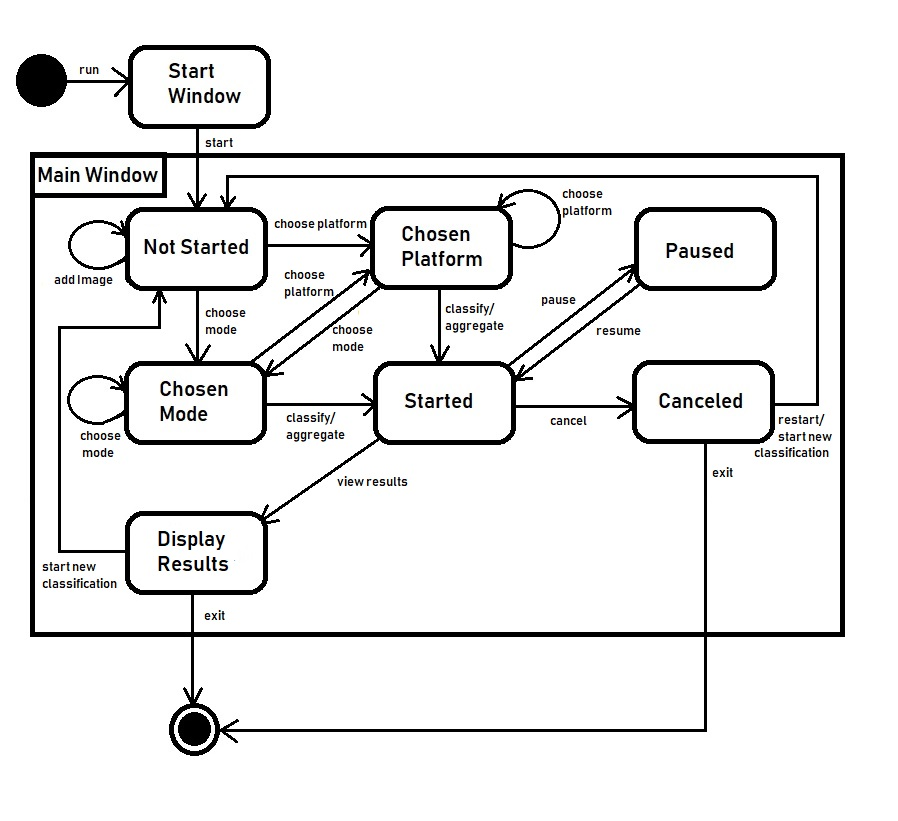
\includegraphics[width=1.0\textwidth]{StateDiag.jpg}
\end{center}

\pagebreak


\end{document}
